\documentclass{beamer}
\usepackage[UTF8]{ctex}
\usepackage{amsmath}
\usepackage{amssymb}
\usepackage{graphicx}
\usepackage{booktabs}
\usepackage{tikz}
\usepackage{algorithm2e}
\usepackage{listings}
\usepackage{xcolor}
\usepackage{hyperref}
\usetikzlibrary{arrows.meta, positioning, shapes,calc}

% Listings Settings
\lstset{
    basicstyle=\small\ttfamily,
    keywordstyle=\color{blue},
    commentstyle=\color{myblue!60!black},
    stringstyle=\color{red},
    showstringspaces=false,
    breaklines=true,
    frame=single,
    tabsize=4,
    numbers=left,
    numberstyle=\tiny\color{gray},
    extendedchars=true,
    inputencoding=utf8,
    literate={…}{{...}}3 {,}{{,}}1 {;}{{;}}1 {(}{{(}}1 {)}{{)}}1 {%}{{\%}}1 {!}{{!}}1 {:}{{:}}1,
}
\usetheme{Madrid}
\definecolor{myteal}{cmyk}{0.5,0,0.15,0}
\definecolor{myyellow}{cmyk}{0,0.2,0.7,0}
\definecolor{myblue}{RGB}{8,51,110}
\definecolor{mygreen}{cmyk}{0.4,0,0.4,0}

\setbeamercolor{structure}{fg=myblue}
\setbeamercolor{title}{fg=white, bg=myblue!90!black}
\setbeamercolor{frametitle}{fg=white, bg=myblue!90!black}
\setbeamercolor{block title}{fg=white, bg=myblue!80!black}
\setbeamercolor{block body}{bg=myblue!5}
\setbeamercolor{itemize item}{fg=myblue}
\setbeamercolor{block title example}{fg=white, bg=myblue!80!black}
\setbeamercolor{block body example}{bg=myblue!5}
\title{自动微分}
\institute{上海师范大学数理学院}
\begin{document}
\frame{\titlepage}
\begin{frame}{目录}
    \tableofcontents
\end{frame}
% ==================================================
\begin{frame}{什么是自动微分?}
\begin{block}{定义}
自动微分(AD)是一种基于链式法则和计算图的数值技术,能够精确高效地计算复杂函数的导数。
\end{block}

\begin{itemize}
\item 不同于数值微分(近似、易出错)和符号微分(表达式爆炸)
\item 现代深度学习框架(PyTorch, TensorFlow)的核心引擎
\item 实现了反向传播的底层机制
\item 支持高阶导数、控制流和自定义梯度
\item 使训练拥有百万级参数的神经网络成为可能
\end{itemize}

\begin{exampleblock}{核心价值}
当我们在PyTorch中调用\texttt{loss.backward()}时,系统能在数秒内计算出所有参数的梯度。自动微分技术是深度学习成功的关键基石。
\end{exampleblock}
\end{frame}

\begin{frame}{自动微分框架}
\begin{center}
\begin{tikzpicture}[
    node distance=1.5cm,
    block/.style={rectangle, draw, fill=blue!20, text width=3cm, text centered, rounded corners, minimum height=1cm},
    arrow/.style={thick,->,>=stealth}
]
\node[block] (input) {输入函数};
\node[block, below of=input] (graph) {构建计算图};
\node[block, below of=graph] (mode) {选择微分模式};
\node[block, right of=mode, node distance=4cm] (method) {前向or反向模式};
\node[block, below of=method] (output) {输出梯度};

\draw[arrow] (input) -- (graph);
\draw[arrow] (graph) -- (mode);
\draw[arrow] (mode) -- (method);
\draw[arrow] (method) -- (output);
\end{tikzpicture}
\end{center}
\end{frame}

% ==================================================
\begin{frame}{微分方法比较}
\begin{block}{总结}
\begin{tabular}{|l|l|l|}
\hline
\textbf{方法} & \textbf{优点} & \textbf{缺点} \\
\hline
数值微分 & 简单易实现 & 精度低,效率差,误差大 \\
符号微分 & 精确结果 & 表达式爆炸,不支持控制流 \\
自动微分 & 精确+高效+完整代码支持 & 实现复杂 \\
\hline
\end{tabular}
\end{block}

\begin{itemize}
\item \textbf{数值微分}: $ f'(x) \approx \frac{f(x+h)-f(x)}{h} $
\begin{itemize}
\item 选择合适$h$困难:太小导致舍入误差,太大导致截断误差
\item $n$维参数计算成本为$O(n)$
\end{itemize}
\item \textbf{符号微分}: 代数推导 $ \frac{d}{dx}\sin(x^2) = 2x\cos(x^2) $
\begin{itemize}
\item 复杂表达式呈指数级增长
\item 无法处理条件语句或循环
\end{itemize}
\item \textbf{自动微分}: 将函数分解为基本运算
\begin{itemize}
\item 机器精度的准确性
\item 与原函数时间复杂度在同一量级
\item 支持任意Python控制流
\end{itemize}
\end{itemize}
\end{frame}

% ==================================================
\section{计算图与链式法则}
\begin{frame}{计算图}
\begin{block}{基本原理}
将函数表示为有向无环图(DAG),节点为变量/操作,边表示数据依赖关系。
\end{block}

\begin{center}
\begin{tikzpicture}[
    node distance=1.5cm,
    input/.style={circle, draw=myblue, thick, fill=white, minimum size=0.9cm},
    op/.style={rectangle, draw=mygreen!70!black, thick, fill=mygreen!10, minimum width=1.2cm, minimum height=0.7cm},
    output/.style={circle, draw=red!70!black, thick, fill=red!5, minimum size=0.9cm},
    edge/.style={->, thick, >=Stealth}
]

% Nodes
\node[input] (x1) {$x_1$};
\node[input, above=1cm of x1] (x2) {$x_2$};
\node[op, above right=0.25cm and 1.5cm of x1] (mul) {$\times$};
\node[op, right=1.5cm of mul] (sin) {$\sin$};
\node[output, right=1.5cm of sin] (y) {$y$};

% Edges
\draw[edge] (x1) -- (mul);
\draw[edge] (x2) -- (mul);
\draw[edge] (mul) -- node[above] {$v_1$} (sin);
\draw[edge] (sin) -- node[above] {$v_2$} (y);

% Caption
\node[below=1cm of mul, text width=6cm, align=center, font=\footnotesize] {
    计算图: $y = \sin(x_1 \times x_2)$ };

\end{tikzpicture}
\end{center}
\end{frame}
% ==================================================
\section{自动微分的两种模式}
\begin{frame}{前向模式}
\begin{block}{工作原理}
\begin{itemize}
\item 从输入到输出传播导数
\item 在计算中间值的同时计算导数
\item 每次前向传播计算一个方向的导数
\end{itemize}
\end{block}

\begin{exampleblock}{数学表达}
对于 $f: \mathbb{R}^n \rightarrow \mathbb{R}^m$,前向模式计算:
$$
J \cdot \mathbf{v} = \begin{bmatrix}
\frac{\partial f_1}{\partial x_1} & \cdots & \frac{\partial f_1}{\partial x_n} \\
\vdots & \ddots & \vdots \\
\frac{\partial f_m}{\partial x_1} & \cdots & \frac{\partial f_m}{\partial x_n}
\end{bmatrix} \begin{bmatrix} v_1 \\ \vdots \\ v_n \end{bmatrix}
$$
\end{exampleblock}

\begin{itemize}
\item 适用于输入维度$n\ll$ 输出维度$m$的情况
\item 通常无需计算出Jacobian矩阵,每次前向传播计算一个方向的导数
\item 无需存储图
\end{itemize}
\end{frame}

\begin{frame}{前向与反向模式对比框架}
\begin{center}
\begin{tikzpicture}[
    node distance=0.5cm and 3.5cm, % vertical and horizontal distance
    block/.style={
        rectangle, 
        draw=myblue!80!black, 
        fill=myblue!10, 
        text width=2.6cm, 
        align=center, 
        rounded corners, 
        minimum height=0.8cm,
        font=\small
    },
    decision/.style={
        diamond, 
        draw=orange!70!black, 
        fill=orange!15, 
        text width=2.2cm, 
        align=center, 
        inner sep=2pt,
        font=\small
    },
    arrow/.style={thick, -Stealth, myblue!80!black},
    label/.style={font=\footnotesize}
]

% ========== 左侧:前向模式 ==========
\node[block] (input1) {输入数据};
\node[block, below=of input1] (forward1) {前向计算 \\ + 前向微分};
\node[block, below=of forward1] (output1) {输出与导数};

% ========== 右侧:反向模式 ==========
\node[block, right=of input1] (input2) {输入数据};
\node[block, below=of input2] (forward2) {前向计算};
\node[block, below=of forward2] (backward) {反向微分};
\node[block, below=of backward] (output2) {输出与梯度};

% ========== 决策节点(居中于两输出下方)==========
\node[decision, below=0cm of $(output1.south)!0.5!(output2.south)$] (decision) {输入维度 $n \ll$ 输出维度 $m$?};

% ========== 连接线 ==========
\draw[arrow] (input1) -- (forward1);
\draw[arrow] (forward1) -- (output1);
\draw[arrow] (input2) -- (forward2);
\draw[arrow] (forward2) -- (backward);
\draw[arrow] (backward) -- (output2);

% 决策连接(从两个输出指向决策)
\draw[arrow] (output1.south) |- (decision.west);
\draw[arrow] (output2.south) |- (decision.east);

% 是/否分支(可选:从决策引出建议)
\node[above=0.2cm of input1, font=\bfseries\small, myblue] {前向模式};
\node[above=0.2cm of input2, font=\bfseries\small, myblue] {反向模式};

% 决策标签
\node[left=0.1cm of decision.west, font=\footnotesize, red] {是};
\node[right=0.1cm of decision.east, font=\footnotesize, blue] {否};

% 建议文本(可选)
\node[below=0.8cm of decision, align=center, font=\small] {%
    \textcolor{red}{适合前向模式} \\
    \textcolor{blue}{适合反向模式}
};

\end{tikzpicture}
\end{center}
\end{frame}
% ==================================================
\begin{frame}{反向模式}
\begin{block}{工作原理}
\begin{itemize}
\item \textbf{前向阶段}: 计算值并记录计算图,\textbf{反向阶段}: 从输出到输入反向传播
\item 一次反向传播计算所有输入的梯度
\end{itemize}
\end{block}

\begin{exampleblock}{数学表达}
对于 $f: \mathbb{R}^n \rightarrow \mathbb{R}^m$,反向模式计算:
$$
\mathbf{v}^T \cdot J = \begin{bmatrix} v_1 & \cdots & v_m \end{bmatrix} \begin{bmatrix}
\frac{\partial f_1}{\partial x_1} & \cdots & \frac{\partial f_1}{\partial x_n} \\
\vdots & \ddots & \vdots \\
\frac{\partial f_m}{\partial x_1} & \cdots & \frac{\partial f_m}{\partial x_n}
\end{bmatrix}
$$
\end{exampleblock}
\begin{itemize}
\item 在调用 torch.autograd.grad 或 tf.gradients 时,若输出非标量,必须通过 grad\_outputs 显式指定 v,以表明你希望对哪些输出分量求导、以及各自的权重。
\item 空间复杂度: $O(\text{图大小})$,时间复杂度:$O(m)$
\end{itemize}
\end{frame}

\begin{frame}{图示反向传播}
\begin{center}

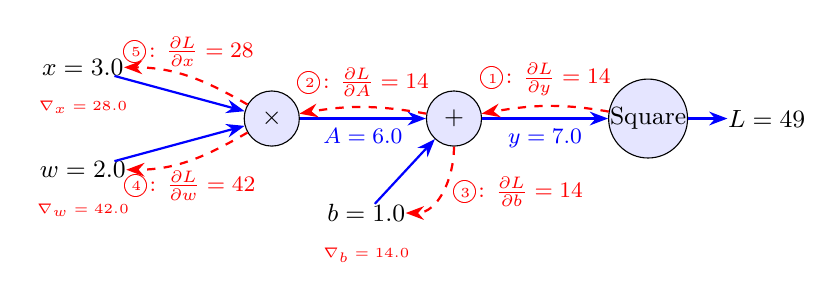
\begin{tikzpicture}[
    node distance=1.2cm,
    every node/.style={align=center},
    op/.style={circle, draw, minimum size=0.7cm, inner sep=0pt, fill=blue!10, font=\small},
    input/.style={inner sep=0pt, font=\small},
    fwdarrow/.style={-Stealth, thick, blue},
    bkarrow/.style={-Stealth, thick, red, dashed},
    label/.style={font=\footnotesize}
]

% 输入节点
\node[input] (x) at (-3.2, 0.65) {$x = 3.0$};
\node[input] (w) at (-3.2, -0.65) {$w = 2.0$};
\node[input] (b) at (0.4, -1.2) {$b = 1.0$};

% 操作节点
\node[op] (mul) at (-0.8, 0) {$\times$};
\node[op, right=1.6cm of mul] (add) {$+$};
\node[op, right=1.6cm of add] (square) {Square};
\node[input, right=0.5cm of square] (loss) {$L = 49$};

% 前向传播
\draw[fwdarrow] (x) -- (mul);
\draw[fwdarrow] (w) -- (mul);
\draw[fwdarrow] (mul) -- node[below, label] {$A = 6.0$} (add);
\draw[fwdarrow] (b) -- (add);
\draw[fwdarrow] (add) -- node[below, label] {$y = 7.0$} (square);
\draw[fwdarrow] (square) -- (loss);

% 反向传播
% ①: ∂L/∂y
\draw[bkarrow] (square) to[out=170,in=10] node[above, label] {\textcircled{\tiny 1}: $\frac{\partial L}{\partial y} = 14$} (add);

% ②: ∂L/∂A
\draw[bkarrow] (add) to[out=170,in=10] node[above, label] {\textcircled{\tiny 2}: $\frac{\partial L}{\partial A} = 14$} (mul);

% ③: ∂L/∂b
\draw[bkarrow] (add) to[out=-90,in=0] node[right, label] {\textcircled{\tiny 3}: $\frac{\partial L}{\partial b} = 14$} (b);

% ④: ∂L/∂w
\draw[bkarrow] (mul) to[out=-150,in=0] node[below, label] {\textcircled{\tiny 4}: $\frac{\partial L}{\partial w} = 42$} (w);

% ⑤: ∂L/∂x
\draw[bkarrow] (mul) to[out=150,in=0] node[above, label] {\textcircled{\tiny 5}: $\frac{\partial L}{\partial x} = 28$} (x);

% 梯度值标注
\node[below=0.2cm of x, color=red, font=\tiny] {$\nabla_x = 28.0$};
\node[below=0.2cm of w, color=red, font=\tiny] {$\nabla_w = 42.0$};
\node[below=0.2cm of b, color=red, font=\tiny] {$\nabla_b = 14.0$};

\end{tikzpicture}

\vspace{0.5cm} % 添加一些空间以分隔上下两部分
\begin{minipage}{\textwidth}
\begin{itemize}
    \item \textbf{Step ①:} $\frac{\partial L}{\partial y} = 14$
    \item \textbf{Step ②:} $\frac{\partial L}{\partial A} = \frac{\partial L}{\partial y} = 14$
    \item \textbf{Step ③:} $\frac{\partial L}{\partial b} = \frac{\partial L}{\partial A} = 14$
    \item \textbf{Step ④:} $\frac{\partial L}{\partial w} = \frac{\partial L}{\partial A} \cdot x = 14 \times 3.0 = 42$
    \item \textbf{Step ⑤:} $\frac{\partial L}{\partial x} = \frac{\partial L}{\partial A} \cdot w = 14 \times 2.0 = 28$
\end{itemize}
\end{minipage}

\end{center}
\end{frame}
% ==================================================
\section{PyTorch autograd}
\begin{frame}[fragile]{PyTorch autograd基础}
\begin{block}{核心组件}
\begin{itemize}
\item \textbf{Tensor}: 基本数据结构,具有\texttt{requires\_grad}属性
\item \textbf{Function}: 记录操作历史,定义前向/反向计算
\item \textbf{Autograd引擎}: 构建计算图并执行反向传播
\end{itemize}
\end{block}

\begin{lstlisting}[language=Python]
import torch
x = torch.tensor(3.0, requires_grad=True)
w = torch.tensor(2.0, requires_grad=True)
b = torch.tensor(1.0, requires_grad=True)
y = w * x + b  # y = 7
loss = y**2    # loss = 49
loss.backward()
print(x.grad)  # dx = 28.0
print(w.grad)  # dw = 42.0
print(b.grad)  # db = 14.0
\end{lstlisting}
\end{frame}

% ==================================================
\begin{frame}{autograd内部机制}
\begin{block}{图构建}
\begin{itemize}
\item 运行张量运算时,都会生成一个对应的 Function 对象。这个对象负责记录这次运算的信息。
\item Function 对象不仅记录了参与运算的张量,还记录了进行的操作类型(如加法、乘法等)
\item 形成图,节点代表 Function 或者是张量,边表示计算顺序。
\item 叶节点(输入)存储梯度;中间节点通常不存储
\end{itemize}
\end{block}

\begin{block}{梯度计算规则}
\begin{itemize}
\item 每个\texttt{Function}定义\texttt{forward}和\texttt{backward}方法
\item \texttt{backward}接收上游梯度并计算下游梯度
\item 梯度累积在叶节点的\texttt{.grad}属性中
\end{itemize}
\end{block}
\end{frame}

\begin{frame}{PyTorch自动微分框架}
\begin{center}
\begin{tikzpicture}[
    node distance=1.5cm,
    block/.style={rectangle, draw, fill=blue!20, text width=3cm, text centered, rounded corners, minimum height=1cm},
    data/.style={rectangle, draw, fill=green!20, text width=2.5cm, text centered, rounded corners, minimum height=0.8cm},
    arrow/.style={thick,->,>=stealth},
    label/.style={font=\footnotesize}
]
% 数据层
\node[data] (tensor) {张量数据};
\node[data, right of=tensor, node distance=4cm] (grad) {损失计算};

% 计算层
\node[block, below of=tensor] (forward) {前向计算和计算图构建};
\node[block, right of=forward, node distance=4cm] (backward) {反向传播};

% 输出层
\node[data, below of=forward] (output) {输出结果};
\node[data, below of=backward] (params) {参数更新};

% 连接线
\draw[arrow] (tensor) -- (forward);
\draw[arrow] (forward) -- (output);
\draw[arrow] (grad) -- (backward);
\draw[arrow] (backward) -- (params);
\draw[arrow, dashed] (params.west) to(tensor.east);
\draw[arrow, dashed] (output.east) to(grad.west);

% 标签
\node[above of=tensor, node distance=0.8cm, label] {数据流};
\node[above of=grad, node distance=0.8cm, label] {梯度流};
\end{tikzpicture}
\end{center}
\end{frame}

% ==================================================
\begin{frame}[fragile]{autograd核心API}
\begin{block}{关键函数}
\begin{itemize}
\item \texttt{torch.autograd.grad(outputs, inputs)}:
\begin{itemize}
\item 显式计算梯度而不修改\texttt{.grad}
\item 支持高阶导数
\end{itemize}
\item \texttt{torch.autograd.functional.jacobian(function, inputs)}:
\begin{itemize}
\item 为多输出函数计算雅可比矩阵
\end{itemize}
\item \texttt{torch.autograd.functional.hessian(function, inputs)}:
\begin{itemize}
\item 计算海森矩阵(二阶导数)
\end{itemize}
\end{itemize}
\end{block}

\begin{lstlisting}[language=Python]
x = torch.tensor(2.0, requires_grad=True)
y = x**3
dy_dx = torch.autograd.grad(y, x, create_graph=True)[0]
d2y_dx2 = torch.autograd.grad(dy_dx, x)[0]
print(dy_dx)   # 12.0
print(d2y_dx2) # 12.0
\end{lstlisting}
\end{frame}

\begin{frame}[fragile]{多输出函数的混合梯度}
\begin{lstlisting}[language=Python]
import torch
x = torch.tensor(2.0, requires_grad=True)
y1 = x ** 2      # y1 = x^2
y2 = x ** 3      # y2 = x^3
# we want: d(y1)/dx  + d(y2)/dx 
# put outputs in a list,grad_outputs is the weights
grad_combined = torch.autograd.grad(
    outputs=[y1, y2],
    inputs=x,
    grad_outputs=[torch.tensor(1.0), torch.tensor(1.0)] 
)[0] #you can also use torch.ones_like([y1, y2])
print(f"Combined gradient = {grad_combined.item():.2f}")
# dy1/dx = 2x = 4
# dy2/dx = 3x^2 = 12
# weighted sum= 1*4 + 1*12 = 16
\end{lstlisting}
\end{frame}

% ==================================================
\begin{frame}[fragile]{梯度控制与优化}
\begin{block}{梯度管理}
\begin{itemize}
\item \texttt{with torch.no\_grad():}: 禁用梯度计算
\begin{itemize}
\item 推理和验证阶段必需
\item 减少内存使用,提高速度
\end{itemize}
\item \texttt{tensor.detach()}: 创建无梯度追踪的副本
\begin{itemize}
\item 阻止梯度流向特定张量
\end{itemize}
\item \texttt{requires\_grad\_()}: 动态启用/禁用梯度
\begin{itemize}
\item 支持微调: 冻结部分层,仅训练其他层
\end{itemize}
\end{itemize}
\end{block}

\begin{lstlisting}[language=Python]
with torch.no_grad():
    prediction = model(x_test) 
for param in model.parameters():
    param.requires_grad_(False)  
model.fc.requires_grad = True  #Two methods are similar,the above one is preferred
\end{lstlisting}
\end{frame}

% ==================================================
\begin{frame}[fragile]{梯度累积与清零}
\begin{block}{正确的梯度更新流程}
\begin{enumerate}
\item \textbf{清零梯度}: \texttt{optimizer.zero\_grad()}
\item \textbf{前向传播}: 计算预测和损失
\item \textbf{反向传播}: \texttt{loss.backward()}
\item \textbf{更新参数}: \texttt{optimizer.step()}
\end{enumerate}
\end{block}

\begin{block}{为什么需要清零梯度?}
\begin{itemize}
\item PyTorch \textbf{默认将梯度求和}(不覆盖)
\item 每次\texttt{backward()}调用将梯度添加到现有\texttt{.grad}值
\item 不清零会导致跨迭代的梯度错误累积
\end{itemize}
\end{block}
\end{frame}
% ==================================================
\begin{frame}[fragile]{训练循环示例}
\begin{block}{标准训练步骤}
\centering
\begin{tikzpicture}[
    node distance=0.8cm,
    mystep/.style={
        rectangle, 
        rounded corners, 
        minimum width=1.5cm, 
        minimum height=0.9cm,
        draw=blue,
        fill=blue!10,
        font=\small
    },
    myarrow/.style={
        ->,
        thick, 
        blue
    }
]
\node (step1) [mystep] {清零梯度};
\node (step2) [mystep, right=of step1] {前向传播};
\node (step3) [mystep, right=of step2] {计算损失};
\node (step4) [mystep, right=of step3] {反向传播};
\node (step5) [mystep, right=of step4] {更新参数};

\draw [myarrow] (step1) -- (step2);
\draw [myarrow] (step2) -- (step3);
\draw [myarrow] (step3) -- (step4);
\draw [myarrow] (step4) -- (step5);
\draw [myarrow, bend right=15] (step5.north) to node[below, font=\tiny] {重复} (step1.north);
\end{tikzpicture}

\vspace{0.3cm}
\begin{lstlisting}[language=Python]
for epoch in range(epochs):
    for batch in dataloader:
        optimizer.zero_grad() 
        outputs = model(inputs)
        loss = criterion(outputs, targets)
        loss.backward()
        optimizer.step()
\end{lstlisting}
\end{block}
\end{frame}
% ==================================================
\begin{frame}[fragile]{自定义梯度函数}
\begin{block}{torch.autograd.Function}
\begin{itemize}
\item 定义自定义操作及其梯度
\item 继承\texttt{torch.autograd.Function}
\item 实现静态\texttt{forward}和\texttt{backward}方法
\item \texttt{forward}: 定义计算
\item \texttt{backward}: 定义梯度计算
\end{itemize}
\end{block}
\end{frame}

\begin{frame}[fragile]{自定义自动微分函数}
\begin{lstlisting}[language=Python]
import torch
from torch.autograd import Function
class Square(Function):
    @staticmethod
    def forward(ctx, input):
        ctx.save_for_backward(input)
        return input ** 2
    @staticmethod
    def backward(ctx, grad_output):
        input, = ctx.saved_tensors
        grad_input = 2 * input * grad_output
        return grad_input
x = torch.tensor(3.0, requires_grad=True)
y = Square.apply(x)
y.backward()
print("x.grad =", x.grad)  
\end{lstlisting}
\end{frame}

% ==================================================
\begin{frame}{自动微分调试}
\begin{block}{常见问题与解决方案}
\begin{itemize}
\item \textbf{梯度消失/爆炸}:
\begin{itemize}
\item 监控梯度范数: \texttt{torch.norm(param.grad)}
\item 应用梯度裁剪: \texttt{torch.nn.utils.clip\_grad\_norm\_}
\end{itemize}
\item \textbf{缺失梯度(None)}:
\begin{itemize}
\item 验证\texttt{requires\_grad=True}已设置
\item 检查计算路径是否中断
\end{itemize}
\item \textbf{原地操作错误}:
\begin{itemize}
\item 避免修改参与梯度计算的张量
\item 优先使用\texttt{x = x + 1}而非\texttt{x += 1}
\end{itemize}
\end{itemize}
\end{block}

\begin{block}{调试工具}
\begin{itemize}
\item \texttt{torch.autograd.detect\_anomaly()}: 捕获异常操作
\item \texttt{torch.autograd.gradcheck()}: 数值验证梯度
\item 检查\texttt{tensor.grad\_fn}: 查看计算图节点
\end{itemize}
\end{block}
\end{frame}

% ==================================================
\begin{frame}[fragile]{ 检查点}
\begin{block}{内存优化}
\begin{itemize}
\item 问题: 大型模型存储计算图消耗过多内存
\item 前向时:只保存 layer2 的输入 x,不保存输出
\item 反向时:用保存的输入 x 重新运行 layer2 的前向
\item 权衡: 以额外计算换取内存减少
\end{itemize}
\end{block}
\begin{lstlisting}[language=Python]
from torch.utils.checkpoint import checkpoint
class MyModel(nn.Module):
    def __init__(self):
        super().__init__()
        self.layer1 = nn.Linear(100, 100)
        self.layer2 = nn.Linear(100, 100)
        self.layer3 = nn.Linear(100, 10)
    def forward(self, x):
        x = self.layer1(x)
        x = checkpoint(self.layer2, x)
        x = self.layer3(x)
        return x
\end{lstlisting}
\end{frame}

\end{document}
